\noindent Este capítulo, constituído pela adaptação do material apresentado no Simpósio de Doutorado do XXIII Ibero-American Conference on Software Engineering\footnote{Versão original disponível em: $<$https://bit.ly/2OLqnwE$>$.}, apresenta os procedimentos que serão utilizados na condução do projeto de doutorado, as atividades que serão desenvolvidas, o cronograma de execução das atividades, assim como, os resultados e contribuições esperados ao término do projeto.


\section{Caracterização da pesquisa}

Sistemas conversacionais representam aplicações que são capazes de processar e emitir a linguagem humana, por meio de texto ou voz \cite{abdul2015survey}. Exemplos comuns dessas aplicações são os assistentes virtuais Siri\footnote{Mais informações disponíveis em $<$https://apple.co/2xjRw0X$>$.}, Google Assistant\footnote{Mais informações disponíveis em $<$http://bit.ly/39GniDQ$>$.} e Cortana\footnote{Mais informações disponíveis em $<$ http://bit.ly/2NnWZfA$>$.} \cite{Laranjo:2018}. Devido às habilidades do processamento de linguagem natural, essas aplicações têm sido estabelecidas para contextos de uso específicos, em diferentes áreas do conhecimento humano. Um dos maiores interesses para o uso desses sistemas é no domínio da educação. Isso pode ser observado em recentes estudos secundários que buscam definir um panorama sobre os sistemas conversacionais produzidos para fins educacionais \cite{hobert2019,io2017}. 

Por intermédio de estudos secundários, é possível observar que os sistemas conversacionais educacionais estão sendo produzidos para apoiar temáticas específicas, como o ensino de física, matemática, computação, engenharias, saúde, dentre outras. Além disso, eles são definidos com propósitos diferentes, na medida em que podem ser usados para solucionar dúvidas de alunos que não compreenderam um assunto, repassar informações que sejam relevantes, fornecer \textit{feedback} para as ações realizadas pelos estudantes, usar discurso motivacional para estimular os estudantes, contribuir com a aquisição de conhecimento do aluno, contribuir com o desenvolvimento de competências sociais, dentre outros. Ainda, eles podem ser definidos para se comportarem como tutores, companheiros de aprendizagem ou estudantes. 

A exploração do uso de sistemas conversacionais pedagógicos em cursos de plataformas \sigla{MOOCs}{\textit{Massive Open Online Courses}} tem se intensificado \cite{aguirre2018}, uma vez que esses cursos possuem uma ampla quantidade e diversidade de estudantes, e nem sempre há um professor disponível para atender aos questionamentos elaborados pelos alunos. Em trabalhos anteriores, o autor explorou o uso desses sistemas como apoio a práticas de ensino baseadas em metodologias ativas, como \textit{Flipped Classroom} \cite{Paschoal:2019}. Apesar de serem estimulados para uso em práticas ativas, esses sistemas também podem ser explorados no ensino tradicional (presencial ou a distância) \cite{krassmann2018}. Nesse sentido, podem ser usados em conjunto com outros recursos educacionais, tais como ambientes virtuais de aprendizagem, redes sociais, mundos virtuais e jogos educacionais.

Dado a versatilidade e aplicabilidade desses sistemas, era esperado que existissem mais estudos na literatura sobre a implantação dos mesmos em práticas educacionais. Todavia, observa-se que a comunidade não tem apresentado relatos sobre a implantação efetiva desses sistemas em cenários de ensino, pois a maioria dos trabalhos tem focado em descrever o desenvolvimento do sistema conversacional pedagógico e tem se distanciado em explorar sua implantação. Foram identificados estudos dedicados a avaliar, por exemplo, a usabilidade de sistemas conversacionais pedagógicos \cite{paschoal2018}. Também, foram encontrados estudos que descrevem o \textit{feedback} dos alunos ou do professor sobre o benefício do agente conversacional \cite{io2017,winkler2018}. No entanto, esses estudos são feitos pelos autores para comprovar alguma funcionalidade \cite{hobert2019}. Portanto, relatos de experiência da implantação dos sistemas conversacionais pedagógicos não são comuns em fóruns de divulgação científica.

Devido a falta de relatórios ou artigos científicos sobre as experiências em implantações desses sistemas, não existem registros de lições a serem aprendidas. Por outro lado, isso pode levar a alguns questionamentos associados à viabilidade das aplicações que estão sendo desenvolvidas. A viabilidade dos sistemas conversacionais poderia ser comprovada por meio de estudos experimentais, como é feito por pesquisadores de engenharia de software quando buscam compreender a viabilidade de técnicas, procedimentos e novas ferramentas \cite{Wohlin}. Trabalhos recentes apontam a falta de sistematização nos estudos que estão sendo produzidos no contexto de sistemas conversacionais \cite{winkler2018}. Sabe-se que isso dificulta o entendimento dos procedimentos e resultados apresentados e a sua replicação \cite{de2016experimentation}. Além disso, cada estudo avalia um aspecto do sistema conversacional, portanto, não há padronização no que é considerado durante a avaliação \cite{hobert2019}. Por exemplo, enquanto alguns pesquisadores avaliam somente aspectos técnicos dos sistemas conversacionais pedagógicos, outros consideram somente as percepções dos estudantes e não observam questões técnicas, como a qualidade da conversa. Desse modo, o entendimento que se tem é que que a comunidade da área ainda não apresenta de maneira clara os elementos que são importantes na avaliação de um sistema conversacional para o ensino.

Essa falta de pesquisas sobre avaliações no contexto de sistemas conversacionais pedagógicos pode ter relação com a falta de procedimentos de apoio à sistematização, como também a falta de conhecimento sobre a necessidade dessa sistematização \cite{io2017}. Como a área é constituída por pesquisadores com formações em diferentes domínios, é possível que as avaliações que estão sendo realizadas tenham relação direta com o que o pesquisador está acostumado a utilizar em trabalhos de sua área. Por exemplo, um pesquisador da área de engenharia pode não conhecer os procedimentos que apoiam a avaliação experimental utilizados por pesquisadores da área da computação.

Neste panorama e considerando que os sistemas conversacionais se diferem dos sistemas de software tradicionais, o desafio desta pesquisa de doutorado é ampliar a sistematização das avaliações sobre a viabilidade dos sistemas conversacionais pedagógicos e padronizar a avaliação conduzida por pesquisadores com diferentes \textit{backgrounds}. Assim, espera-se propor um framework de apoio para avaliações experimentais de sistemas conversacionais pedagógicos de modo que a viabilidade, qualidade e outros requisitos de interesse possam ser avaliados com maior confiabilidade. O objetivo é padronizar as avaliações experimentais de modo que os resultados possam ser melhor comparados. Busca-se promover direcionamentos para apoiar pesquisadores a definir avaliações sistemáticas de sistemas conversacionais pedagógicos, concentrando nos diferentes estágios de uma avaliação sistemática – a saber: planejamento, operação, execução e divulgação.

\section{Justificativa}

Os sistemas conversacionais emergem como sistemas de software com potencial para solucionar ou minimizar problemas associados ao ensino e a aprendizagem, uma vez que flexibilizam a interação entre usuário-computador e podem estar disponíveis para uso a todo momento, isto é, 24 horas por dia e 7 dias por semana \cite{Jain:2018}. Com base nessa premissa, muitos pesquisadores vêm tirando proveito desses sistemas para propor soluções às problemáticas que permeiam o âmbito educacional. No entanto, somente a proposta e o desenvolvimento desses sistemas não garante que os problemas estão sendo solucionados. 

De acordo com \citeonline{Shull} e  \citeonline{Travassos:2002}, os produtos de software não deveriam ser apenas propostos, desenvolvidos ou apresentados para venda sem experimentação e validação. Na visão de \citeonline{Basili:1998}, só é possível verificar se o entendimento atual sobre a temática está correto por meio de estudos experimentais. Desse modo, acredita-se que só é possível averiguar se sistemas conversacionais pedagógicos conseguem solucionar os problemas para os quais são propostos por meio da condução de estudos experimentais.

O paradigma experimental tem sido adotado e adaptado por diversas linhas de investigação dentro da Ciência da Computação, tais como Sistemas Operacionais \cite{FORTIER2003331} e Engenharia de Software \cite{Wohlin}. No âmbito da Engenharia de Software existem algumas definições para os propósitos da experimentação. \citeonline{Conradi:2001} descrevem que a experimentação auxilia a construir uma base de conhecimento confiável, permitindo reduzir as incertezas sobre quais as teorias, ferramentas e metodologias são adequadas. Adicionalmente, a experimentação elimina suposições errôneas e oferece suporte para orientar a teoria nas direções promissoras de pesquisa \cite{Conradi:2001}.

Apesar da experimentação estar bem estabelecida na área da engenharia de software, a condução de experimentos em outras áreas ainda não é uma prática habitual. De acordo com \citeonline{Kitchenham:2002}, algumas áreas de pesquisa têm dificuldade em realizar estudos experimentais. Em virtude disso, existem estudos que discutem sobre a necessidade de adaptar os modelos já estabelecidos e consolidados em outras áreas ou desenvolver modelos específicos para o domínio de investigação. Considerando as necessidades intrínsecas da área e tipos de aplicações, muitas áreas têm concentrado esforços para o estabelecimento de diretrizes, processos e \textit{frameworks} de apoio a experimentação. Em \citeonline{Vos:2012}, por exemplo, os autores apresentam um framework para pesquisa de experimental sobre técnicas e ferramentas de teste de software. Já na pesquisa de \citeonline{Sheard:2009}, por exemplo, os autores mencionam sobre a necessidade de adequação de um modelo de experimentação para ambientes de apoio ao ensino de programação. 

Em decorrência do atual estado da arte sobre os sistemas conversacionais pedagógicos, acredita-se que é necessário oferecer apoio metodológico, visando estimular a condução de estudos experimentais na área. Supõe-se que o apoio metodológico aumentará o rigor da pesquisa na área e contribuirá com a adesão de procedimentos sistemáticos durante a condução desses estudos. Adicionalmente, é necessário apoiar a replicação dos experimentos, estimulando a geração de pacotes de dados experimentais com conjunto de informações importantes para a replicação, buscando facilitar o compartilhamento e reúso de materiais produzidos, adotados e gerados durante a condução de experimentos.

\section{Solução proposta}

Considerando que o projeto de pesquisa conduzido no contexto do doutorado envolve a investigação e o estabelecimento de um framework para apoiar o planejamento, operação, condução e relato de estudos experimentais sobre sistemas conversacionais pedagógicos, busca-se:

\begin{enumerate}

   \item Estabelecer um vocabulário de experimentação para que pesquisadores conduzam e reportem seus estudos utilizando conceitos e terminologias comuns. O vocabulário é importante porque a comunidade de pesquisa que trabalha com sistemas conversacionais pedagógicos provêm de diferentes áreas do conhecimento humano e precisa conseguir utilizar a mesma linguagem para compartilhar os resultados de suas avaliações.

    \item Definir um corpo de conhecimento sobre variáveis e métricas. O corpo de conhecimento possibilitará ao usuário final do framework  reconhecer quais as variáveis que podem ser controladas e não podem ser controladas na condução de experimentos sobre sistemas conversacionais pedagógicos, dando ênfase a dois tipos de variáveis, a saber: variáveis dependentes e variáveis independentes. Nessa etapa, serão investigadas e classificadas as variáveis dependentes que são de interesse para estes sistemas (\textit{e.g.}, eficácia, desempenho, qualidade das respostas, qualidade da interface, funcionalidade, percepção e contribuição para o que se propõe). Adicionalmente, será definido, com base na literatura, um conjunto de possíveis métricas para essas variáveis.

   \item Produzir diretrizes para que os pesquisadores ao projetarem as avaliações experimentais possam identificar as possíveis ameças à validade do estudo. Essas diretrizes devem apresentar recomendações para evitá-las.

   \item Propor um guia de experimentação para a condução de experimentos sobre sistemas conversacionais pedagógicos. Nessa perspectiva, o guia indicará atividades que devem ser planejadas e realizadas durante a condução do experimento. O guia tem o propósito de orientar o usuário final do framework na realização das atividades para o planejamento e realização do experimento. Adicionalmente, o guia deverá indicar quais são as informações relevantes que devem compor o relatório do experimento.
   
   \item Desenvolver um agente conversacional com conhecimentos sobre experimentação. A intenção do agente será auxiliar o pesquisador a definir os procedimentos necessários para executar e reportar um estudo experimental sobre sistemas conversacionais educacionais. Portanto, o usuário poderá interagir em língua natural com o mecanismo de apoio e resolver suas dúvidas sobre o processo de experimentação.  
   
\end{enumerate}
 
Os artefatos descritos constituirão o framework metodológico, que também pode ser interpretado como um framework de pesquisa, cuja definição é baseada em \citeonline{Basili:1998} e consiste em uma estrutura organizacional que pode ser oferecida como uma meta genérica definida para ser instanciada em experimentos e em uma família de experimentos\footnote{Uma família de experimentos engloba um grupo de avaliações experimentais similares que estudam o mesmo objeto de estudo, considerando diferentes variações \cite{Basili:1998}.},  um conjunto de variáveis  para  ser explorado e usado no processo experimental, uma coleção de métricas para serem utilizadas como medidas às variáveis selecionadas no projeto experimental, etc. A Figura \ref{framework} apresenta uma ilustração de como o framework será constituído. Destaca-se o agente conversacional ao centro da figura, indicando que o modelo de conhecimento do agente conversacional contemplará o conhecimento sobre cada artefato.

\begin{figure}[!htb]
\centering
\caption{Uma visão geral do framework metodológico}
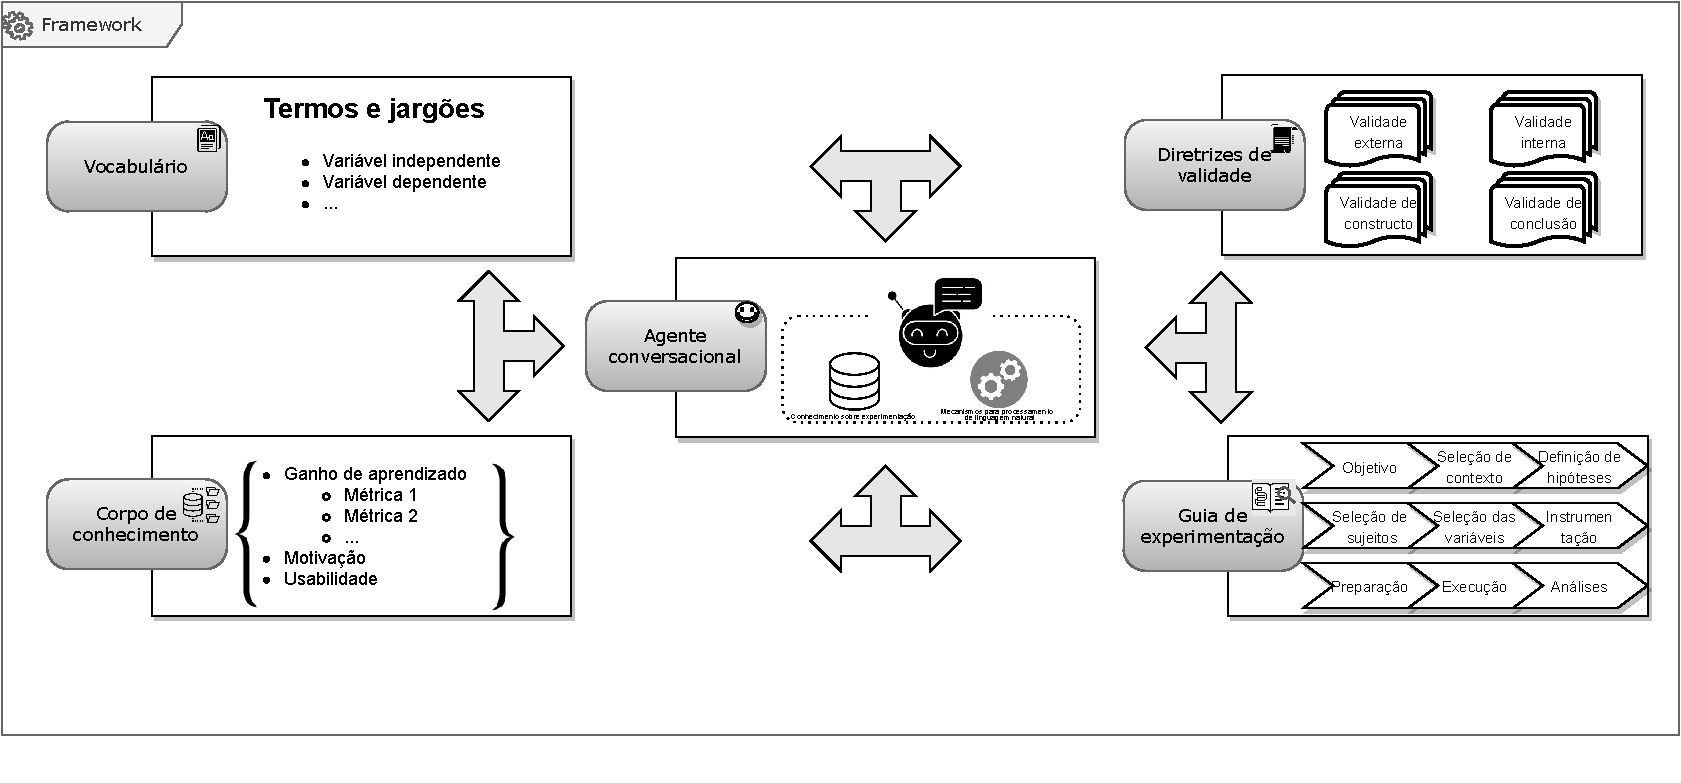
\includegraphics[width=0.95\textwidth]{Figuras/desenho.pdf}
\label{framework}
\fautor
\end{figure}
 
\section{Método de pesquisa} 

O framework metodológico proposto será constituído por um conjunto de artefatos. Dessa forma, a abordagem epistemológico-metodológica \textit{Design Science Research} será utilizada para caracterizar a pesquisa. Essa abordagem tem sido explorada em estudos que envolvem o estabelecimento de artefatos para um determinado contexto a fim de melhorar algo ou resolver um dado problema, especialmente em áreas como Engenharia de Software e Sistemas de Informação \cite{wieringa2014}. Os artefatos devem ser interpretados de forma ampla pela \textit{Design Science Research}, podendo ser constructos, algoritmos, métodos e frameworks.  

Um artefato é desenvolvido visando contribuir para melhor realização de um objetivo. Nesse sentido, a meta definida para este estudo, organizada no \textit{template} apresentado por \citeonline{wieringa2014}, consiste em: \underline{melhorar} os estudos experimentais sobre sistemas conversacionais educacionais, \underline{por meio de} um framework metodológico, \underline{que satisfaça} aspectos inerentes a validade de um experimento, replicação e generalização de resultados, \underline{para que} pesquisadores possam planejar, conduzir, executar e reportar de modo sistematizado os estudos experimentais. %Portanto, \underline{o artefato} discutido é o framework metodológico e \underline{o contexto} deste estudo é sistemas conversacionais educacionais.

Como envolve o desenvolvimento de um artefato (ou um conjunto de artefatos), espera-se que um ciclo de engenharia seja seguido. Para tanto, pode ser utilizado o ciclo de design apresentado em \citeonline{wieringa2014} ou o processo definido por \citeonline{Peffers:2007}. Neste estudo, será utilizado o processo definido por \citeonline{Peffers:2007}, que é composto por seis atividades. Vale salientar que a terminologia de cada atividade muda dependendo da base bibliográfica utilizada, mas as tarefas realizadas e a proposta principal são mantidas em cada interpretação do \textit{Design Science Research}. Em particular, as tarefas consideradas neste estudo são ilustradas pela Figura \ref{processoDSR}. Elas serão feitas, preferencialmente, seguindo um fluxo sequencial, com momentos de revisão e aprimoramento dos resultados.

\begin{figure}[!htb]
\centering
\caption{Processo de Design Science Research}
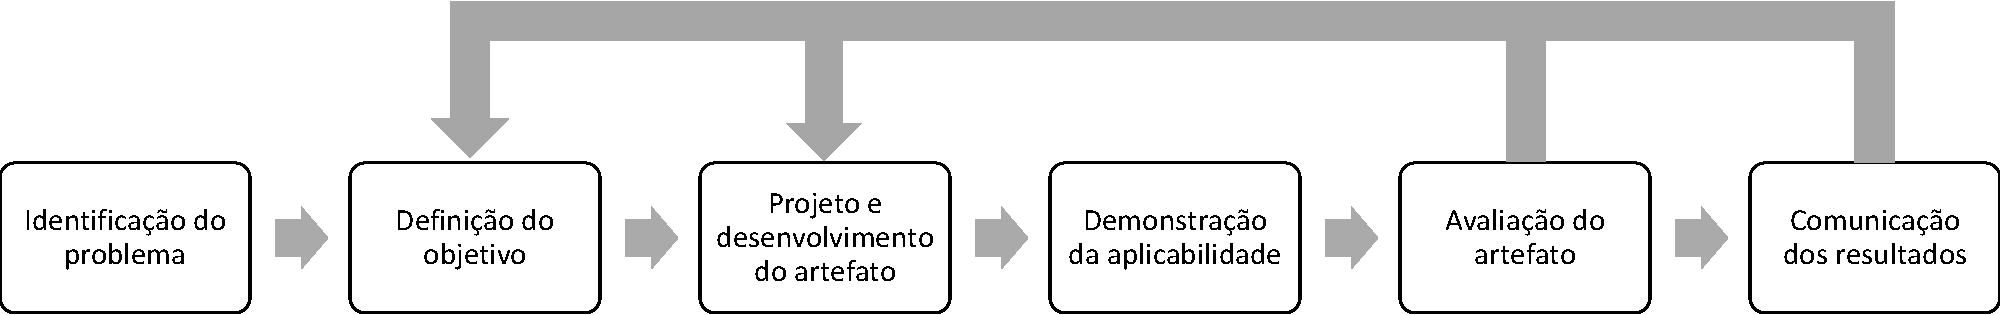
\includegraphics[width=0.95\textwidth]{Figuras/ProcessoDSR.pdf}
\label{processoDSR}
\fadaptada{Peffers:2007}
\end{figure}

Cada uma das atividades ilustradas na Figura \ref{processoDSR} é descrita a seguir:

 \begin{itemize}
    \item \textit{Identificação do problema:} a primeira tarefa envolve a investigação do problema, o reconhecimento das necessidades de uma temática e o valor de uma solução para esse problema;
    \item \textit{Definição do objetivo:} a segunda tarefa envolve a determinação do objetivo da pesquisa e identificação da viabilidade da solução proposta;
    \item \textit{Projeto e desenvolvimento do artefato:} a terceira tarefa envolve o estabelecimento propriamente dito do artefato, desde a especificações até a implementação;
    \item \textit{Demonstração da aplicabilidade:} a quarta tarefa envolve a demonstração da aplicação por meio de uma ou mais instanciações;
    \item \textit{Avaliação do artefato:} a quinta tarefa envolve a avaliação do artefato, considerando diferentes tipos de pesquisa (\textit{i.e.}, qualitativa ou quantitativa) e métodos (\textit{e.g.}, survey, estudo de caso, experimento controlado, dentre outros);  Salienta-se que a avaliação do artefato deve considerar os efeitos do artefato implementado. Portanto, pode englobar desdobramentos de pesquisas para compreender os efeitos gerados pelo artefato, até mesmo o entendimento sobre como o artefato causa tais efeitos;
    \item \textit{Comunicação dos resultados:} a sexta e última tarefa envolve o compartilhamento dos resultados alcançados para a comunidade de interesse, por meio de artigos científicos e relatórios técnicos.

 \end{itemize}
 
Como a pesquisa envolve vários artefatos que constituem o framework metodológico, a abordagem \textit{Design Science Research} será adotada em cada artefato e, portanto, no framework como um todo. A Tabela \ref{tab:atividades} descreve como cada tarefa do processo de \citeonline{Peffers:2007} está sendo utilizado na concepção do framework em sua totalidade. Apesar da adoção da abordagem, cada artefato será projetado e avaliado de formas distintas, considerando diferentes teorias para seu embasamento e métodos para avaliação. Por exemplo, um mapeamento sistemático da literatura pode ser utilizado para reforçar a necessidade de vocabulário, diretrizes para validade e um corpo de conhecimento de variáveis e métricas. 

\begin{table}[h]
\centering
\caption{Descrição das etapas de concepção do framework metodológico}
\begin{tabular}{p{5cm}p{10cm}}
\hline
\textbf{Atividade}                    & \textbf{Descrição}                                                                                                                                                                                                                                            \\ \hline
\multirow{4}{17em}{Identificação do problema}            & A identificação do problema aconteceu por meio de revisão bibliográfica, considerando principalmente estudos secundários realizados nos últimos anos sobre sistemas conversacionais educacionais                                                              \\
\multirow{4}{17em}{Definição do objetivo}                 & O objetivo foi definido no decorrer desta seção, considerando uma recomendação para descrição precisa de metas para pesquisas que utilizam a abordagem epistemológica \textit{Design Science Research}                                                              \\
\multirow{2}{17em}{Projeto e desenvolvimento} \multirow{3}{17em}{do artefato} & O projeto e desenvolvimento do artefato englobará a definição de cinco artefatos. Cada artefato será estabelecido de uma maneira, considerando suas diferentes características                                                                                \\
\multirow{2}{17em}{Demonstração da} \multirow{3}{17em}{aplicabilidade}        & Serão projetados exemplos com instancias do framework para sistemas conversacionais educacionais com diferentes requisitos e objetivos pedagógicos                                                                                                            \\
\multirow{5}{17em}{Avaliação do artefato}                 & O framework será avaliação por meio de um estudo experimental com pesquisadores que têm trabalhado com sistemas conversacionais pedagógicos, buscando reconhecer a completude e corretude dos designs de estudos experimentais projetados pelos pesquisadores \\
\multirow{2}{17em}{Comunicação dos resultados}            & Artigos científicos serão produzidos e apresentados em conferências e periódicos da temática                                                                                                                                                                  \\ \hline
\end{tabular}
\label{tab:atividades}

\end{table}

\section{Definição das atividades e cronograma}

Levando em consideração o método e objetivo descrito no decorrer da seção anterior, bem como a motivação e justificativas levantadas, apresenta-se, a seguir, as principais atividades a serem realizadas e que constituem o desenvolvimento deste projeto de doutorado:

\begin{itemize}

\item \textbf{Mapeamento das avaliações existentes:} inicialmente, serão localizados estudos que reportam a avaliação de sistemas conversacionais pedagógicos. Apesar desses não apresentarem avaliação sistemática, por meio deles é possível começar a identificar variáveis e métricas que poderão fazer parte do \textit{framework}. Para mapeá-los será replicado o mapeamento sistemático feito pelo autor e descrito em \citeonline{Paschoal:2020FIE}, incluindo critérios que permitem a seleção de estudos primários sobre sistemas conversacionais que abordem algum tipo de avaliação.

\item \textbf{Definição de um vocabulário:} a replicação do mapeamento permitirá ter um entendimento mais detalhado sobre o estado real de uso de conceitos e terminologias. Assim, considerando os estudos de \citeonline{Wohlin} e \citeonline{Shull}, será definido um vocabulário para experimentação de sistemas conversacionais pedagógicos. 

\item \textbf{Agrupamento de métodos e abordagens de avaliação:} um mapeamento sistemático sobre métodos e abordagens que são definidos para apoiar a avaliação de sistemas conversacionais está previsto. Espera-se que esse mapeamento possibilite a identificação de métricas, medidas e instrumentos que possam apoiar a definição do corpo de conhecimento sobre variáveis e métricas. 

\item \textbf{Construção do corpo de conhecimento:} Após a realização dos estudos secundários, as informações extraídas nos estudos selecionados devem ser reunidas, organizadas e disponibilizadas para acesso público como base de pesquisa e consulta. O corpo de conhecimento será definido considerando uma instanciação da abordagem de \citeonline{Vos:2012}.

\item \textbf{Reconhecimento e escrita das ameças à validade:} a definição das diretrizes para os pesquisadores reportarem ameaças à validade será inspirada em procedimentos adotados no estudo de \citeonline{de2016experimentation}. 

\item \textbf{Proposta de um guia de apoio à experimentação:} o guia para apoiar a experimentação de sistemas conversacionais pedagógicos será planejado considerando o processo experimental de \citeonline{Wohlin}. Esse guia ilustrará procedimentos e apresentará exemplos de planejamentos de experimentos.  

\item \textbf{Concepção do agente conversacional:} a concepção do agente conversacional levará em conta os artefatos estabelecidos ao longo da pesquisa para modelar o conhecimento do agente. Além disso, as experiências do autor no desenvolvimento desse tipo de software, que foram compartilhadas em estudos anteriores \cite{Paschoal:2019, paschoal2018}, serão utilizadas.

\item \textbf{Avaliação do framework:} após a definição dos artefatos, o \textit{framework} de pesquisa proposto será avaliado. A avaliação será realizado por meio de um estudo experimental conduzido com pesquisadores que trabalham com sistemas conversacionais pedagógicos.

\item \textbf{Condução de experimentos no contexto do TOB--STT: } ao passo que o framework seja construído, almeja-se utilizar os artefatos para projetar e conduzir estudos experimentais com a intenção de aprimorar o agente TOB--STT e compreender o seu impacto no ensino de teste de software.

\end{itemize}


Além disso, de acordo com as exigências do Programa de Pós-Graduação em Ciências de Computação e Matemática Computacional (CCMC), para obtenção do título de Doutor, outras atividades são obrigatórias, a saber:

\begin{itemize}

\item \textbf{Obtenção dos créditos para o curso de doutorado:} de acordo com o regulamento vigente do Programa de Pós-Graduação em Ciências da Computação e Matemática Computacional, alunos regulares no curso de doutorado devem cumprir pelo menos 44 créditos em disciplinas oferecidas pelo programa para o depósito da dissertação. Atualmente, o aluno cumpriu 45 créditos, obtendo conceito A em todas as disciplinas. A Tabela \ref{tab:creditos} apresenta algumas informações sobre as disciplinas cursadas.

\begin{table}[h]
\centering
\caption{Obtenção de créditos em disciplinas}
\label{tab:creditos}
\begin{tabular}{p{7cm}ccc}
\hline
\textbf{Disciplina} & \textbf{Carga horária} & \textbf{Créditos} & \textbf{Conceito} \\ \hline
Fundamentos do Gerenciamento Ágil de Projetos & 180 & 12 & A \\
Validação e Teste de Software & 180 & 12 & A \\
Interação Usuário-Computador I: Fundamentos & 120 & 8 & A \\
Interação Usuário-Computador II: Prática & 60 & 4 & A \\
Empreendedorismo & 90 & 6 & A \\
Atividades de Cultura e Extensão Universitária na Pós-Graduação & 30 & 2 & A \\
Tópicos em Computação e Matemática Computacional II & 15 & 1 & A \\ \hline
\end{tabular}
\end{table}

\item \textbf{Exame de proficiência em língua estrangeira:} no prazo de 18 meses do início do curso de doutorado é exigido ao aluno a comprovação de proficiência na língua inglesa, considerando pontuação e exames definidos pelo programa em conjunto com a Pró-reitora de Pós-graduação. O aluno comprovou proficiência no primeiro mês do curso, cumprindo esse requisito.

\item \textbf{Redação da monografia de qualificação e defesa no exame de qualificação:} de acordo com o regimento do programa, todo aluno deve passar por um exame de qualificação, a ser realizado em até 18 meses após o início do curso. Para tanto, o aluno redigiu esta monografia e apresentará até maio de 2021 a uma banca composta por três professores doutores, presidiada pelas orientadoras do estudante.

\item \textbf{Elaboração de artigos científicos:} os resultados obtidos ao longo do estudo devem ser organizados e escritos em formato de artigos científicos. Conforme o regimento do programa, são esperados artigos publicados em conferências nacionais e internacionais e em journal de relevância para a linha de pesquisa do programa. Ao menos, a coordenação do programa exige a publicação de um journal.

\item \textbf{Redação da tese e defesa do doutorado:} ao final dos 48 meses de matriculado do aluno, o aluno deve depositar e apresentar a tese, redigita em português ou inglês, que conterá os resultados de pesquisa obtidos ao longo do período. A defesa deverá ser feito em idioma equivalente ao texto redigido, em uma banca constituída por três professores doutores.

\end{itemize}

O cronograma apresentado no Quadro \ref{tab:schedule} especifica a atividade e o período em que a mesma será realizada.

%\onehalfspace

\newcommand{\y}{\rule{13,5pt}{5pt}}
\newcommand{\x}{\hspace*{5pt}}
\setlength{\tabcolsep}{0pt}
\begin{quadro}[!ht] 
\footnotesize
\caption{Cronograma}
\begin{tabular}{|l|c|c|c|c|c|c|c|c|c|c|c|c|c|c|c|c|}
  \cline{2-17}
  \multicolumn{1}{l|}{} & \multicolumn{3}{c|}{2019} & \multicolumn{4}{c|}{2020}  & \multicolumn{4}{c|}{2021} & \multicolumn{4}{c|}{2022}& \multicolumn{1}{c|}{2023}\\
  \cline{2-17}
  \multicolumn{1}{c|}{\textbf{Atividades}} &
  \rotatebox{90}{Abr-Jun\hspace{2pt}} &
  \rotatebox{90}{Jul-Set\hspace{2pt}} &
  \rotatebox{90}{Out-Dez\hspace{2pt}} &
  \rotatebox{90}{Jan-Mar\hspace{2pt}} &
  \rotatebox{90}{Abr-Jun\hspace{2pt}} &
  \rotatebox{90}{Jul-Set\hspace{2pt}} &
  \rotatebox{90}{Out-Dez\hspace{2pt}} &
  \rotatebox{90}{Jan-Mar\hspace{2pt}} &
  \rotatebox{90}{Abr-Jun\hspace{2pt}} &
  \rotatebox{90}{Jul-Set\hspace{2pt}} &
  \rotatebox{90}{Out-Dez\hspace{2pt}} &
  \rotatebox{90}{Jan-Mar\hspace{2pt}} &
  \rotatebox{90}{Abr-Jun\hspace{2pt}} &
  \rotatebox{90}{Jul-Set\hspace{2pt}} &
  \rotatebox{90}{Out-Dez\hspace{2pt}} &
  \rotatebox{90}{Jan-Mar\hspace{2pt}} 
  %\rotatebox{90}{Nov-Dec\hspace{2pt}} &
  %\rotatebox{90}{Jan-Feb\hspace{2pt}} &
  %\rotatebox{90}{Mar-Apr\hspace{2pt}} &
  %\rotatebox{90}{May-Jun\hspace{2pt}} &
  %\rotatebox{90}{Jul-Aug\hspace{2pt}} &
  %\rotatebox{90}{Sep-Oct\hspace{2pt}} &
  %\rotatebox{90}{Nov-Dec\hspace{2pt}} &
  %\rotatebox{90}{Jan-Feb\hspace{2pt}} 
  \\
  \hline
  Mapeamento das avaliações        
  & \x & \x & \x & \y & \x & \x & \x & \y & \y & \x & \x & \x & \x & \x & \x & \x  \\
  \hline
  Vocabulário           
  & \x & \x & \x & \x & \x & \x & \x & \x & \y & \y & \x & \x & \x & \x & \x & \x  \\
  \hline
  Agrupamento de métodos e abordagens  
  & \x & \x & \x & \x & \x & \x & \x & \x & \x & \x & \y & \x & \x & \x & \x & \x  \\
  \hline
  Corpo de conhecimento
  & \x & \x & \x & \x & \x & \x & \x & \x & \x & \x & \y & \x & \x & \x & \x & \x  \\
  \hline
  Escrita das ameaças
  & \x & \x & \x & \x & \x & \x & \x & \x & \x & \x & \x & \y & \x & \x & \x & \x  \\
  \hline
  Guia de experimentação
  & \x & \x & \x & \x & \x & \x & \x & \x & \x & \x & \x & \x & \y & \x & \x & \x  \\
  \hline
  Agente conversacional
  & \x & \x & \x & \x & \x & \x & \x & \x & \x & \x & \x & \x & \x & \y & \x & \x  \\
  \hline
  Avaliação do framework
  & \x & \x & \x & \x & \x & \x & \x & \x & \x & \x & \x & \x & \x & \x & \y & \x  \\
  \hline
  Experimentos no TOB--STT
  & \x & \x & \y & \x & \x & \y & \x & \x & \x & \y & \x & \x & \y & \x & \y & \y  \\
  \hline  
  Créditos do curso          
  & \y & \y & \y & \x & \x & \x & \x & \x & \x & \x & \x & \x & \x & \x & \x & \x  \\
  \hline
  Proficiência  
  & \y & \x & \x & \x & \x & \x & \x & \x & \x & \x & \x & \x & \x & \x & \x & \x  \\
  \hline
  Qualificação          
  & \x & \x & \x & \x & \x & \x & \y & \y & \x & \x & \x & \x & \x & \x & \x & \x  \\
  \hline
  Artigos
  & \x & \x & \y & \x & \y & \y & \x & \x & \y & \x & \y & \x & \y & \x & \x & \y  \\
  \hline
  Tese          
  & \x & \x & \x & \x & \x & \x & \x & \y & \x & \x & \x & \x & \x & \x & \x & \y  \\
  \hline
\end{tabular}
 \label{tab:schedule}
\end{quadro}


\section{Resultados esperados}

Com o desenvolvimento deste projeto de doutorado espera-se obter as seguintes contribuições:

\begin{enumerate}

\item Aprofundar os estudos sobre avaliações no contexto de sistemas conversacionais educacionais.

\item Fortalecer o entendimento que a comunidade vinculada aos sistemas conversacionais educacionais tem sobre avaliações sistemáticas.

\item Aprimorar a condução de estudos experimentais por intermédio de um corpo de conhecimento e um guia de experimentação.

\item Possibilitar o desenvolvimento de sistemas conversacionais com mais qualidade, uma vez que a partir dos estudos experimentais é possível analisar adequadamente a viabilidade das soluções propostas.

\item Ampliar a credibilidade dos sistemas conversacionais como mecanismo de apoio ao ensino.

\item Consolidar o agente conversacional TOB--STT como um mecanismo eficaz de apoio ao ensino de teste de software.

\item Auxiliar na formação de recursos humanos em Engenharia de Software considerando desenvolver um projeto de iniciação científica atrelado ao projeto em questão e desdobramento de novos projetos de mestrado e doutorado.

\end{enumerate}


